\newpage
\section{Experimentos y Análisis de Resultados}
\label{sec:experimentos}

\subsection{Configuración Experimental y Parámetros}

Para evitar redundancias, se remite al Punto \ref{sec:formulacion} para la definición formal del problema, los conjuntos de datos (IBEX 35, S\&P 100 y S\&P 500) y las restricciones sobre las posiciones de los activos. A continuación se especifican los detalles experimentales necesarios para la reproducibilidad y la comparación empírica.

\subsubsection*{Condiciones de ejecución}

\begin{itemize}
    \item \textbf{Ejecuciones independientes:} 50 por algoritmo y mercado. Semilla base $seed=42$, incrementada secuencialmente ($42+i$).
    \item \textbf{Criterio de parada global:} máximo de 10\,000 evaluaciones de la función objetivo para todos los algoritmos estocásticos.
    \item \textbf{Datos y partición temporal:} entrenamiento 2015--2024 y prueba 2025 para todos los algoritmos.
\end{itemize}

\subsubsection*{Parámetros de los algoritmos de trayectoria}

\begin{itemize}
    \item \textbf{Enfriamiento Simulado:} $\mu=0.2$, $\phi=0.3$, $T_f=10^{-3}$, $max\_vecinos=10 \cdot n$ y $max\_exitos = n$ (equivalente a $0.1\cdot max\_vecinos$).
    \item \textbf{BMB e ILS:} 5 arranques por ejecución. La BL interna se acota a 2000 evaluaciones por arranque.
    \item \textbf{ILS:} tasa de mutación del 20\% para la perturbación de la mejor solución.
    \item \textbf{ILS-ES:} misma perturbación que ILS, sustituyendo la BL por ES en cada arranque.
\end{itemize}

\subsubsection*{Parámetros de la búsqueda local en el algoritmo de referencia (P2)}

El mejor algoritmo de la Práctica 2 identificado en las ejecuciones es \textbf{AM-Best}. Se mantiene como referencia en tablas y análisis con los parámetros configurados en \texttt{config.cfg}:

\begin{itemize}
    \item \textbf{Frecuencia:} cada 10 generaciones.
    \item \textbf{Aplicación:} BL aplicada al 10\% superior (AM-Best).
    \item \textbf{Intensidad:} máximo 100 evaluaciones por BL; ratio de transferencia reducido al 15\%.
\end{itemize}

\subsection{Resultados Numéricos y Boxplots}

Se muestran las tablas exigidas por el guion, incluyendo Greedy, Random y BL (P1), el mejor algoritmo de P2 (AM-Best), y las técnicas de trayectoria de P3 (BMB, ILS, ES, ILS-ES). Los valores provienen de la salida de ejecución en \texttt{salida.txt}.

\begin{table}[H]
\centering
\caption{Resultados numéricos -- IBEX 35}
\label{tab:global-ibex35}
\resizebox{\textwidth}{!}{%
\begin{tabular}{lcccccc}
\hline
Algoritmo & Fitness(2015--2024) & Fitness(2025) & Beneficio(2025) & Std & Evaluaciones & Tiempo (s) \\
\hline
Greedy & -4.794 & -3.227 & -0.033 & 0.000 & 1 & 0.000 \\
Random & -4.911 & -3.305 & 0.052 & 0.091 & 10000 & 0.025 \\
BL & -4.614 & -3.116 & 0.021 & 0.039 & 1078 & 0.001 \\
Mejor P2 (AM-Best) & -4.490 & -3.083 & 0.033 & 0.000 & 10000 & 0.007 \\
BMB & -4.574 & -3.107 & 0.023 & 0.020 & 5403 & 0.004 \\
ILS & -4.606 & -3.115 & 0.021 & 0.036 & 4349 & 0.003 \\
ES & -4.653 & -3.126 & 0.020 & 0.010 & 3244 & 0.002 \\
ILS-ES & -4.649 & -3.127 & 0.020 & 0.014 & 3130 & 0.002 \\
\hline
\end{tabular}
}
\end{table}

\begin{table}[H]
\centering
\caption{Resultados numéricos -- S\&P 100}
\label{tab:global-sp100}
\resizebox{\textwidth}{!}{%
\begin{tabular}{lcccccc}
\hline
Algoritmo & Fitness(2015--2024) & Fitness(2025) & Beneficio(2025) & Std & Evaluaciones & Tiempo (s) \\
\hline
Greedy & -3.305 & -3.791 & 0.100 & 0.000 & 1 & 0.000 \\
Random & -3.400 & -4.080 & 0.079 & 0.041 & 10000 & 0.069 \\
BL & -3.116 & -3.890 & 0.097 & 0.084 & 4351 & 0.023 \\
Mejor P2 (AM-Best) & -2.816 & -3.734 & 0.100 & 0.008 & 10000 & 0.036 \\
BMB & -3.006 & -3.863 & 0.092 & 0.046 & 10000 & 0.065 \\
ILS & -3.114 & -3.888 & 0.097 & 0.082 & 9926 & 0.055 \\
ES & -3.300 & -3.987 & 0.088 & 0.030 & 1828 & 0.011 \\
ILS-ES & -3.311 & -3.991 & 0.085 & 0.038 & 2863 & 0.017 \\
\hline
\end{tabular}
}
\end{table}

\begin{table}[H]
\centering
\caption{Resultados numéricos -- S\&P 500}
\label{tab:global-sp500}
\resizebox{\textwidth}{!}{%
\begin{tabular}{lcccccc}
\hline
Algoritmo & Fitness(2015--2024) & Fitness(2025) & Beneficio(2025) & Std & Evaluaciones & Tiempo (s) \\
\hline
Greedy & -3.370 & -3.909 & 0.024 & 0.000 & 1 & 0.000 \\
Random & -3.648 & -4.364 & 0.019 & 0.044 & 10000 & 0.678 \\
BL & -3.428 & -4.330 & 0.004 & 0.154 & 9645 & 0.603 \\
Mejor P2 (AM-Best) & -2.735 & -3.898 & 0.017 & 0.037 & 10000 & 0.367 \\
BMB & -3.263 & -4.189 & 0.010 & 0.078 & 10000 & 1.071 \\
ILS & -3.434 & -4.312 & 0.005 & 0.146 & 10000 & 0.689 \\
ES & -4.062 & -4.760 & 0.010 & 0.101 & 308 & 0.016 \\
ILS-ES & -4.035 & -4.761 & 0.007 & 0.092 & 546 & 0.030 \\
\hline
\end{tabular}
}
\end{table}

A continuación se presentan los boxplots correspondientes a los algoritmos de la Práctica 3 para cada mercado:

\begin{figure}[H]
\centering
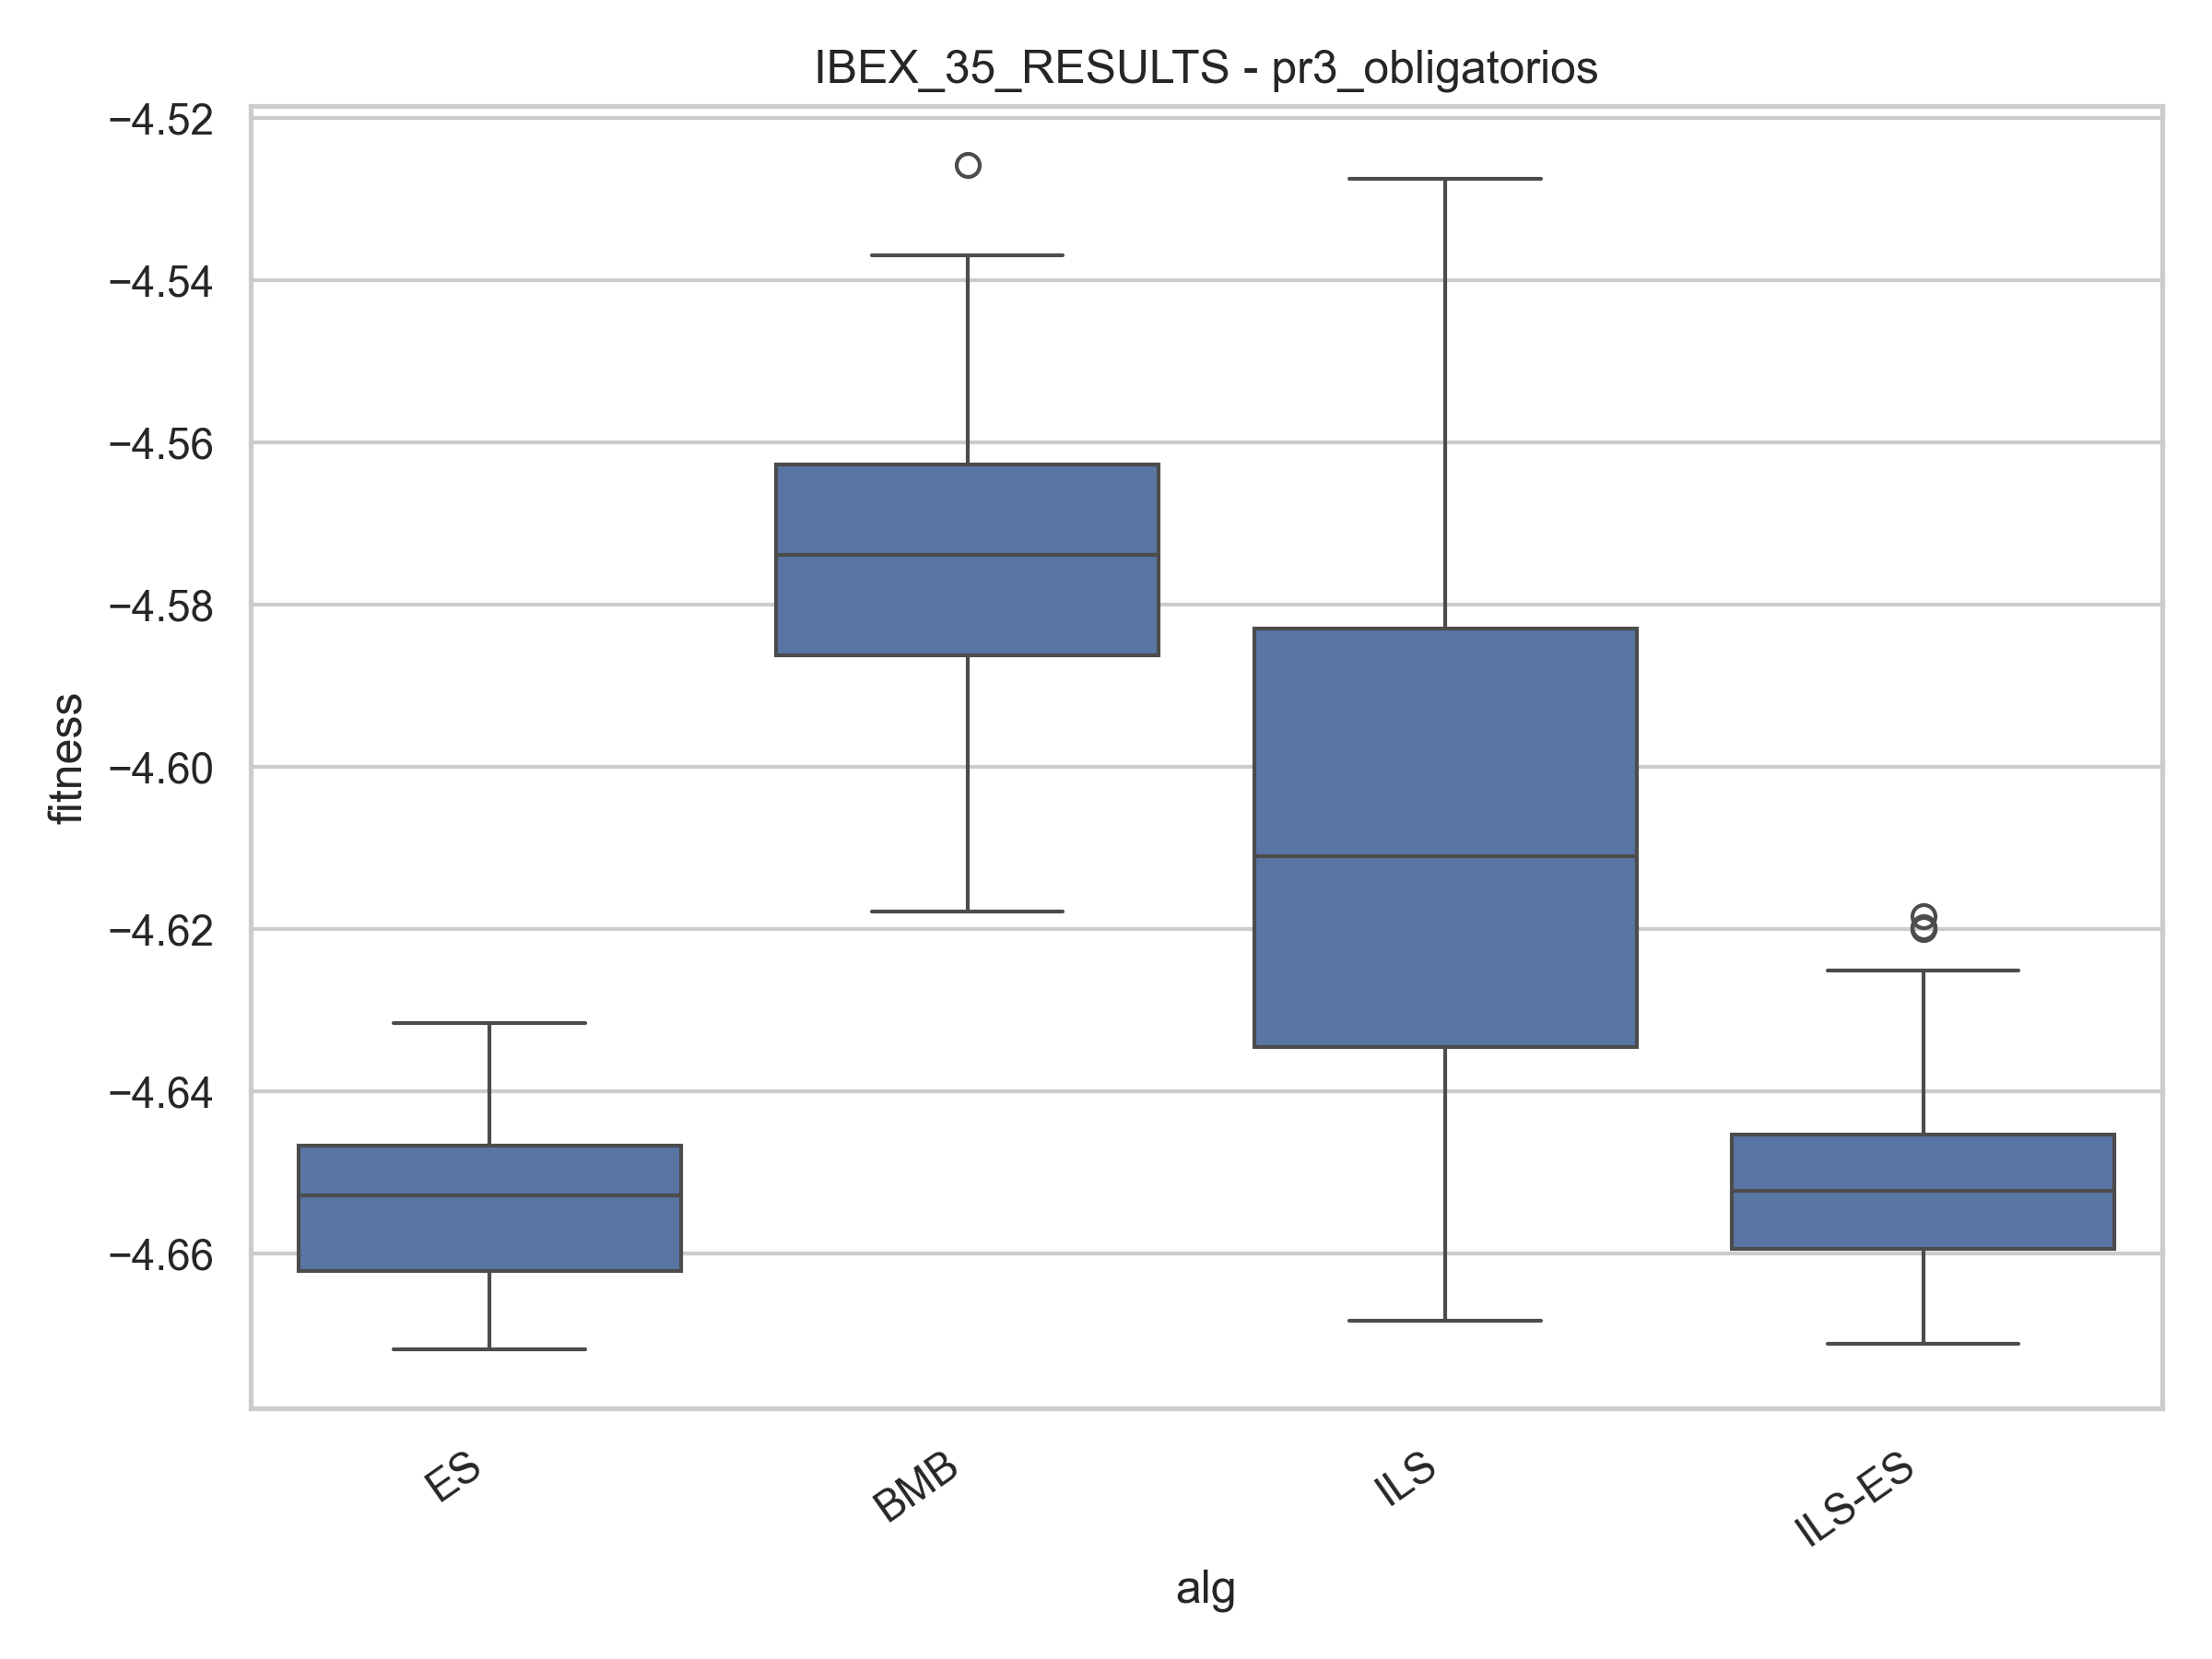
\includegraphics[width=0.8\textwidth]{figuras/IBEX_35_RESULTS_pr3_obligatorios.png}
\caption{Boxplots algoritmos trayectoria (Práctica 3) -- IBEX 35.}
\label{fig:pr3-obligatorios-ibex}
\end{figure}

\begin{figure}[H]
\centering

\includegraphics[width=0.8\textwidth]{\detokenize{figuras/S&P_100_RESULTS_pr3_obligatorios.png}}
\caption{Boxplots algoritmos trayectoria (Práctica 3) -- S\&P 100.}
\label{fig:pr3-obligatorios-sp100}
\end{figure}

\begin{figure}[H]
\centering

\includegraphics[width=0.8\textwidth]{\detokenize{figuras/S&P_500_RESULTS_pr3_obligatorios.png}}
\caption{Boxplots algoritmos trayectoria (Práctica 3) -- S\&P 500.}
\label{fig:pr3-obligatorios-sp500}
\end{figure}

\subsection{Análisis de Resultados}

\subsubsection*{Comparativa con los algoritmos de referencia (P1/P2)}

En los tres mercados, el mejor algoritmo de la Práctica 2 (AM-Best) domina en fitness medio, tanto en entrenamiento como en test, confirmando que las técnicas poblacionales con intensificación selectiva son más eficaces cuando hay presupuesto suficiente de evaluaciones. En IBEX 35, AM-Best mejora a BL en $\approx 0.124$ puntos de fitness y reduce la dispersión (Std $=0.000$). En S\&P 100 y S\&P 500, la ventaja es aún mayor, señalando que la búsqueda poblacional explora de forma más global en alta dimensión. Esto justifica su uso como algoritmo de referencia frente a las trayectorias de P3.

\subsubsection*{ES frente a BL: exploración estocástica vs. explotación local}

ES obtiene fitness medios inferiores a BL en los tres mercados (Tablas \ref{tab:global-ibex35}--\ref{tab:global-sp500}), pero con tiempos de ejecución sustancialmente menores y desviaciones típicas moderadas. En IBEX 35 la diferencia de calidad es pequeña, y en S\&P 500 se observa un outlier superior (Figura~\ref{fig:pr3-obligatorios-sp500}), lo que confirma la capacidad del criterio de Metrópolis para escapar ocasionalmente a mejores cuencas de atracción que BL.

\subsubsection*{BMB frente a ILS: reinicio aleatorio vs. reinicio informado}

BMB supera a ILS en fitness medio en los tres mercados, y además presenta menor dispersión (Std). En este problema, el reinicio puramente aleatorio parece más efectivo que la perturbación del 20\%, posiblemente porque la mutación no altera suficientemente la estructura de la cartera en alta dimensión, conduciendo al ILS a valles similares. Los boxplots refuerzan esta idea: en S\&P 100 aparece un outlier inferior en BMB, pero también una mayor estabilidad en el resto de ejecuciones.

\subsubsection*{ILS-ES: hibridación y sensibilidad}

ILS-ES muestra un comportamiento mixto: mejora a ES en IBEX 35 y S\&P 500, pero es ligeramente peor en S\&P 100. La combinación de saltos de ILS con ES permite ocasionalmente encontrar soluciones de alta calidad (dos outliers superiores en IBEX 35 y uno en S\&P 100), aunque también introduce sensibilidad a los parámetros de enfriamiento, reflejada en un outlier inferior en S\&P 500.

\subsubsection*{Análisis de outliers (indicaciones\_analisis)}

Las figuras de boxplot muestran patrones destacados que conviene justificar:
\begin{itemize}
    \item \textbf{IBEX 35:} un outlier superior en BMB y dos outliers superiores en ILS-ES.
    \item \textbf{S\&P 100:} un outlier inferior en BMB y un outlier superior en ILS-ES.
    \item \textbf{S\&P 500:} un outlier superior en ES y un outlier inferior en ILS-ES.
\end{itemize}
Estos casos se corresponden con ejecuciones donde el criterio de aceptación probabilístico (ES) o las perturbaciones de ILS cambian la trayectoria hacia cuencas de atracción atípicas, elevando o degradando el fitness respecto a la media.

\subsection{Estudio de Eficiencia}

\begin{figure}[H]
\centering
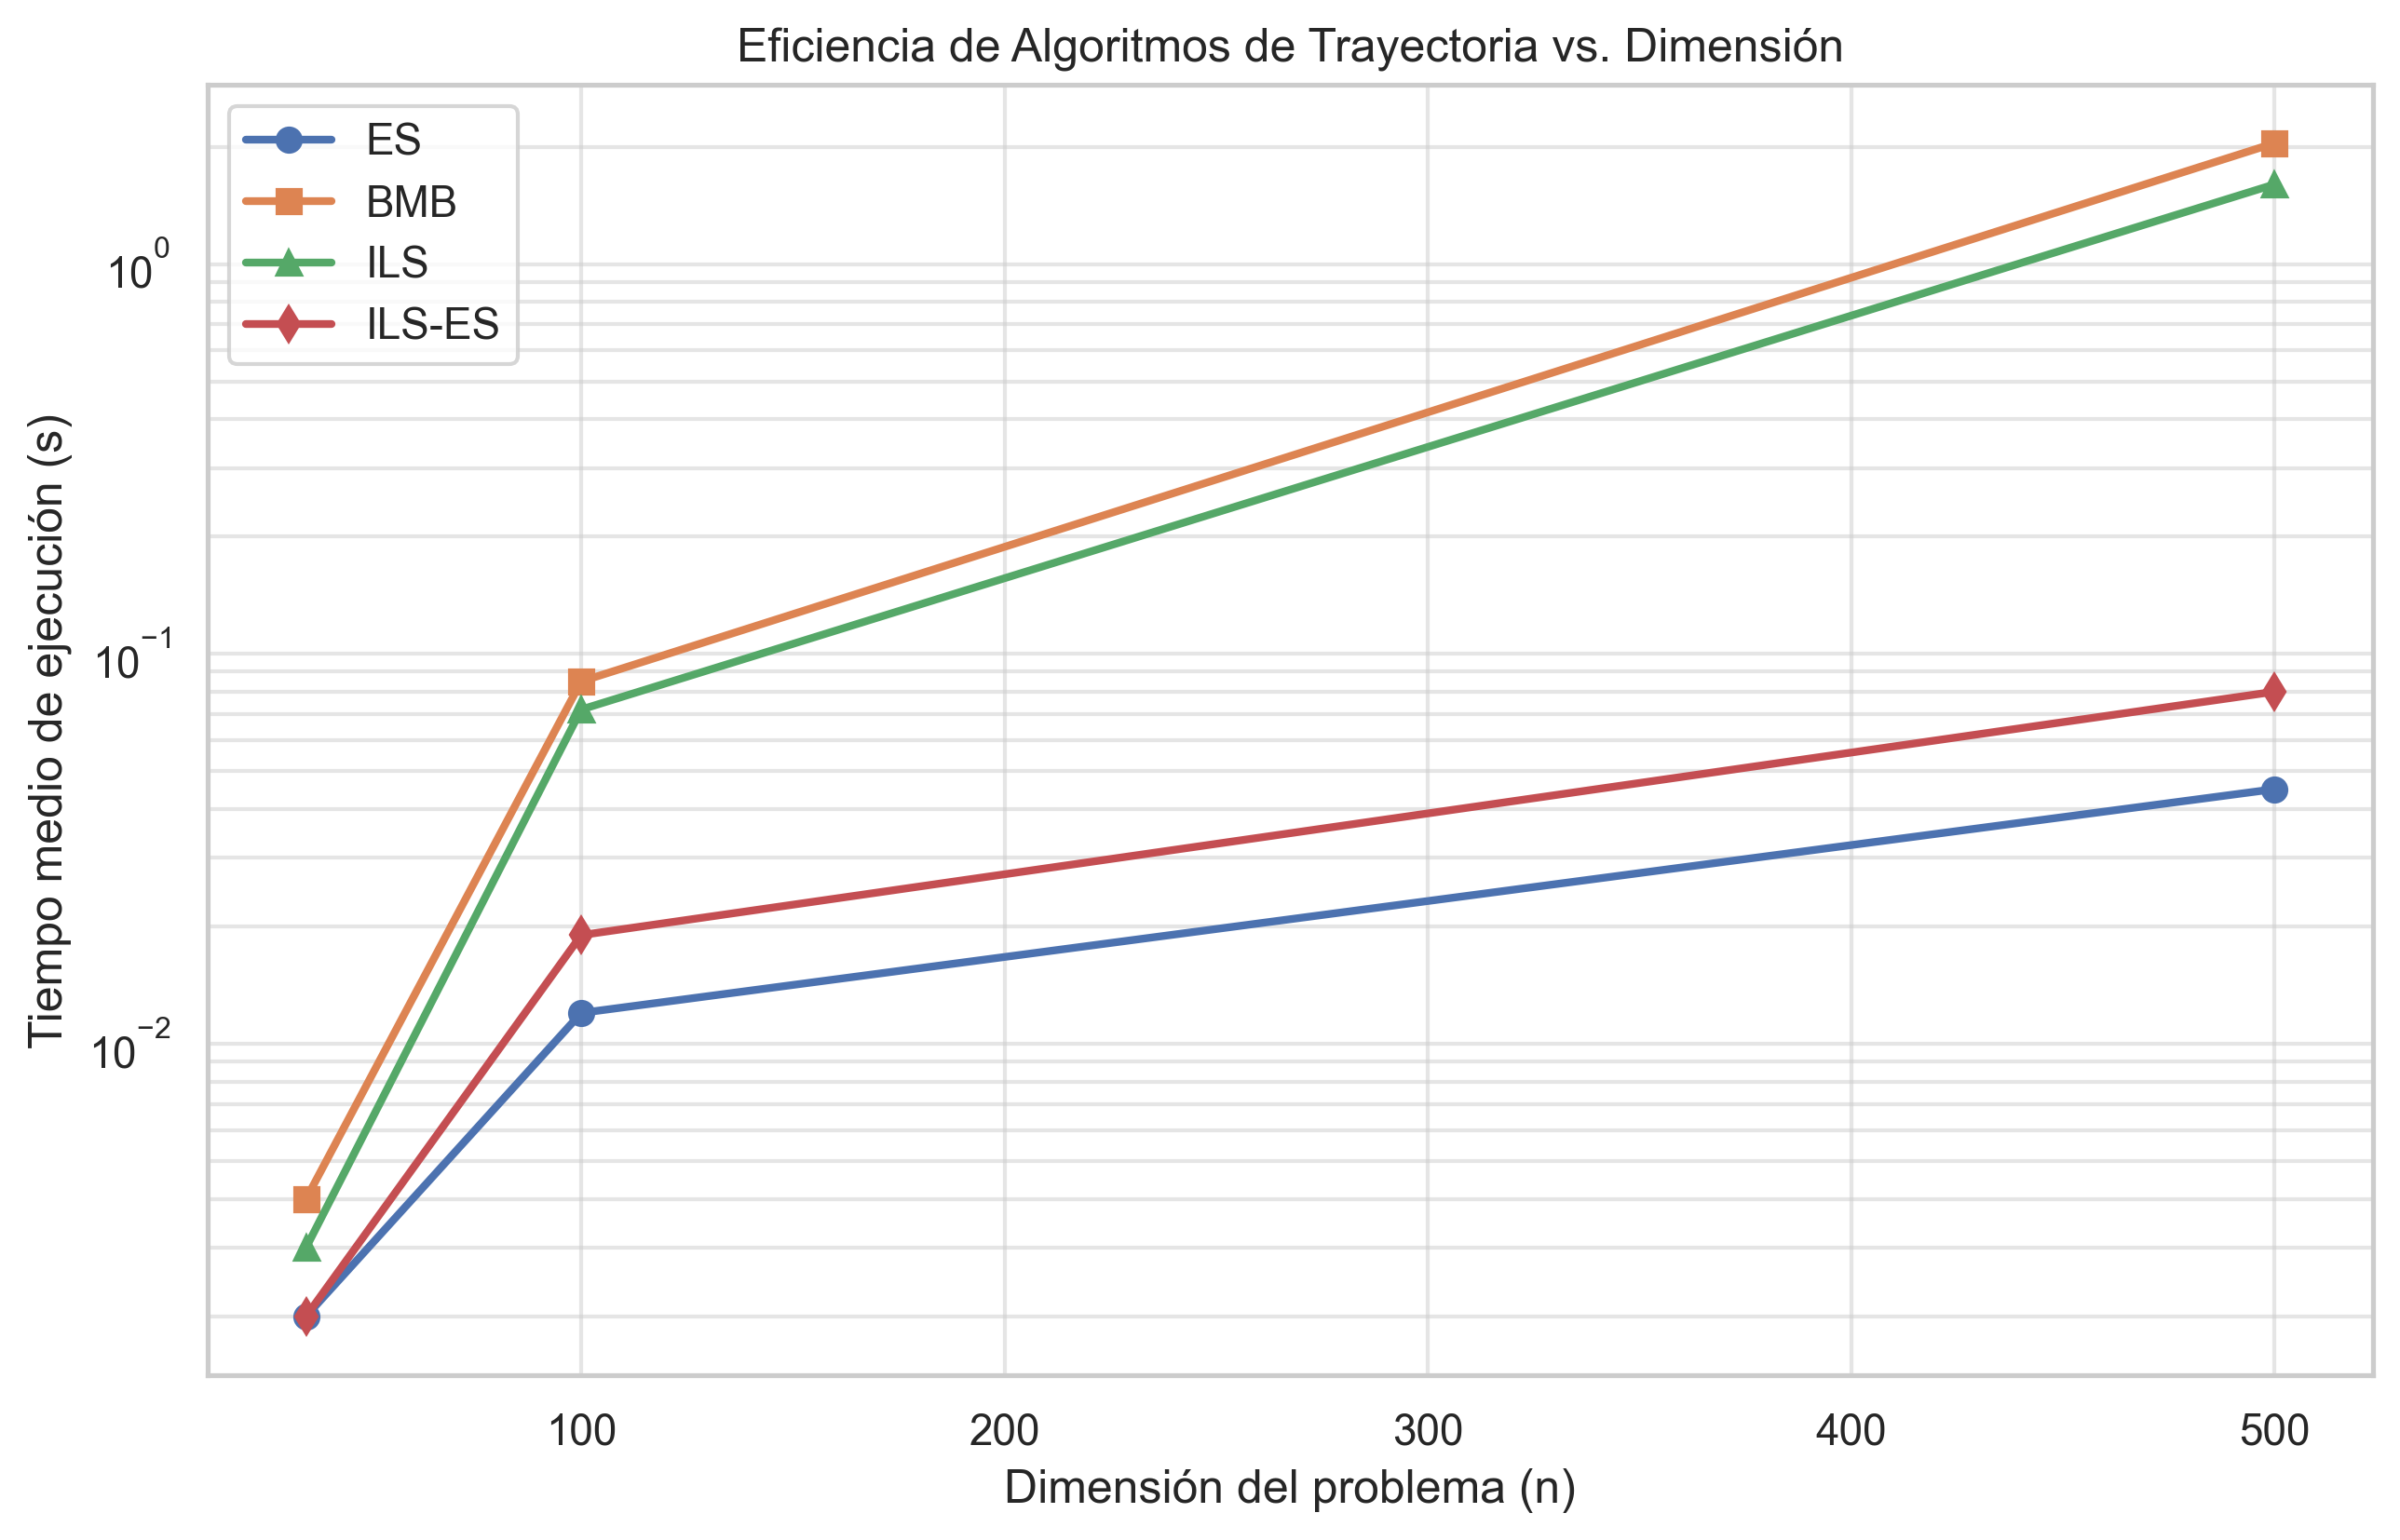
\includegraphics[width=0.8\textwidth]{figuras/eficiencia_trayectoria.png}
\caption{Figura 4: Eficiencia de los algoritmos de trayectoria según la dimensión del problema.}
\label{fig:eficiencia-trayectoria}
\end{figure}

La Figura~\ref{fig:eficiencia-trayectoria} muestra que ES e ILS-ES son los más rápidos en las tres dimensiones, debido a que consumen menos evaluaciones internas por arranque. En cambio, BMB e ILS presentan mayor coste temporal por la repetición de BL (5 arranques de 2000 evaluaciones), lo que incrementa notablemente el tiempo en S\&P 500. Esta diferencia confirma el trade-off clásico entre intensificación (BL repetida) y coste computacional.
